\begin{figure}[t]
\centering
\definecolor{vanRed}{HTML}{C5635F}
\definecolor{r2sGreen}{HTML}{2EB58F}
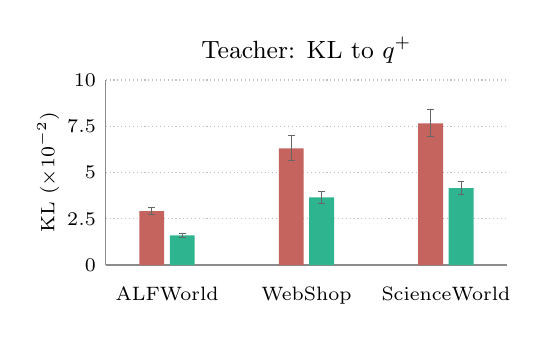
\begin{tikzpicture}
\begin{axis}[
  width=5.1cm, height=2.35cm, scale only axis, ybar, bar width=9pt, bar shift auto, enlarge x limits=0.22,
  symbolic x coords={ALFWorld,WebShop,ScienceWorld}, xtick=data, ymin=0, ymax=10, ytick={0,2.5,5,7.5,10},
  axis lines*=left, axis line style={black!45}, tick style={draw=none}, ytick pos=left,
  ymajorgrids, grid style={densely dotted, black!25}, every tick label/.append style={font=\scriptsize},
  ylabel={KL ($\times 10^{-2}$)}, ylabel style={font=\scriptsize, yshift=-4pt},
  title={Teacher: KL to $q^{+}$}, title style={font=\small, yshift=-3pt, text height=1.8ex, text depth=0.3ex},
  error bars/y dir=both, error bars/y explicit, error bars/error bar style={black!60, line width=0.4pt},
  error bars/error mark options={rotate=90, black!60, mark size=1.2pt},
]
\addplot[fill=vanRed, draw=none] coordinates {(ALFWorld,2.91) += (0,0.22) -= (0,0.20) (WebShop,6.31) += (0,0.67) -= (0,0.67) (ScienceWorld,7.66) += (0,0.74) -= (0,0.69)};
\addplot[fill=r2sGreen, draw=none] coordinates {(ALFWorld,1.60) += (0,0.10) -= (0,0.10) (WebShop,3.65) += (0,0.33) -= (0,0.32) (ScienceWorld,4.15) += (0,0.36) -= (0,0.34)};
\end{axis}
\end{tikzpicture}
\hfill
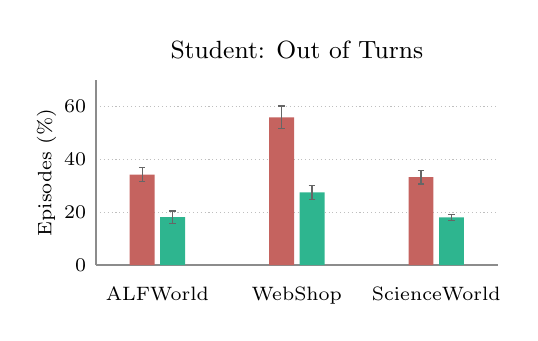
\begin{tikzpicture}
\begin{axis}[
  width=5.1cm, height=2.35cm, scale only axis, ybar, bar width=9pt, bar shift auto, enlarge x limits=0.22,
  symbolic x coords={ALFWorld,WebShop,ScienceWorld}, xtick=data, ymin=0, ymax=70, ytick={0,20,40,60},
  axis lines*=left, axis line style={black!45}, tick style={draw=none}, ytick pos=left,
  ymajorgrids, grid style={densely dotted, black!25}, every tick label/.append style={font=\scriptsize},
  ylabel={Episodes (\%)}, ylabel style={font=\scriptsize, yshift=-4pt},
  title={Student: Out of Turns}, title style={font=\small, yshift=-3pt, text height=1.8ex, text depth=0.3ex},
  error bars/y dir=both, error bars/y explicit, error bars/error bar style={black!60, line width=0.4pt},
  error bars/error mark options={rotate=90, black!60, mark size=1.2pt},
]
\addplot[fill=vanRed, draw=none] coordinates {(ALFWorld,34.18) +- (0,2.65) (WebShop,55.87) +- (0,4.28) (ScienceWorld,33.24) +- (0,2.59)};
\addplot[fill=r2sGreen, draw=none] coordinates {(ALFWorld,18.10) +- (0,2.36) (WebShop,27.53) +- (0,2.66) (ScienceWorld,18.02) +- (0,1.13)};
\end{axis}
\end{tikzpicture}

{\scriptsize \tikz[baseline=-0.4ex]{\fill[vanRed] (0,-0.02) rectangle (0.3,0.16);}\,Vanilla OPD\quad\tikz[baseline=-0.4ex]{\fill[r2sGreen] (0,-0.02) rectangle (0.3,0.16);}\,\method{}}
\caption{\textbf{Repair moves the teacher toward its informed targets, and its student runs out of turns about half as often.} Left: each teacher's top-16 KL to $q^{+}$ on held-out states, with 95\% goal-bootstrap intervals. Right: held-out episodes that end unfinished at the turn budget, mean $\pm$ std over three decodes.}
\label{fig:scorer-effect}
\end{figure}
